\documentclass[11pt,a4paper]{article}
\usepackage[margin=1in]{geometry}
\usepackage{graphicx}
\usepackage{booktabs}
\usepackage{longtable}
\usepackage{caption}
\usepackage{hyperref}
\usepackage{array}
\usepackage{float}
\usepackage{listings}
\usepackage{xcolor}
\usepackage{amsmath}

\captionsetup{font=small,labelfont=bf}

\lstset{
  language=Python,
  basicstyle=\ttfamily\small,
  keywordstyle=\color{blue}\bfseries,
  commentstyle=\color{gray},
  stringstyle=\color{red},
  breaklines=true,
  showstringspaces=false,
  frame=single,
  numbers=left,
  numberstyle=\tiny,
  captionpos=b
}

\title{Experiment 5: Multilayer Perceptron (MLP) \\ \large Multi-class Classification Report}
\author{Prepared by: \textbf{Sreeram GM} \\
Course / Lab: Experiment 5}
\date{\today}

\begin{document}
\maketitle
\tableofcontents
\bigskip

\section{Aim}
Implement a Multilayer Perceptron (MLP) for multi-class classification on the provided image dataset, perform grid-based hyperparameter search, evaluate the best model on a held-out test set, and present metrics and plots.

\section{Dataset}
\begin{itemize}
  \item Dataset root (Colab / Google Drive): \texttt{/content/drive/MyDrive/colabdata/dataset}
  \item Contents:
    \begin{itemize}
      \item \texttt{Img/} : folder containing image files.
      \item \texttt{*.csv} : CSV file mapping image filenames to labels.
    \end{itemize}
  \item Summary (from experiment run):
    \begin{itemize}
      \item Loaded \(X\): \textbf{(3410, 784)}, \(y\): \textbf{(3410,)}
      \item Number of classes: \textbf{62}
      \item Data splits: Train: \textbf{2182}, Validation: \textbf{546}, Test: \textbf{682}
    \end{itemize}
\end{itemize}

\section{Preprocessing}
\begin{enumerate}
  \item Mount Google Drive and locate dataset folder.
  \item Load CSV and auto-detect filename and label columns.
  \item Resolve image file paths robustly (search in \texttt{Img/} and dataset root).
  \item For each image:
    \begin{itemize}
      \item Convert to grayscale (PIL `L`).
      \item Resize to \textbf{28$\times$28}.
      \item Normalize pixel values to [0,1].
      \item Flatten to a vector of length 784.
    \end{itemize}
  \item Use \texttt{LabelEncoder} to obtain integer labels.
  \item Use stratified splits: first train/test (80/20), then train/val from train.
\end{enumerate}

\section{Implementation}
Below are the key code sections used in the experiment. The full runnable code (single Colab cell) is included in the appendix.

\subsection{Mounting and CSV / Image loading}
\begin{lstlisting}[caption={Mount Drive and auto-detect CSV + load filenames}]
# Mount Drive and set dataset paths
from google.colab import drive
drive.mount('/content/drive')

DATASET_ROOT = '/content/drive/MyDrive/colabdata/dataset'
IMG_FOLDER = DATASET_ROOT + '/Img'
import os, pickle
print("Dataset root:", DATASET_ROOT)
print("Image folder:", IMG_FOLDER)
print("Exists?:", os.path.exists(DATASET_ROOT), os.path.exists(IMG_FOLDER))

# find CSV file
def find_csv_file(dataset_root):
    candidates = [f for f in os.listdir(dataset_root) if f.lower().endswith('.csv')]
    if not candidates:
        raise FileNotFoundError(f"No CSV file found in {dataset_root}.")
    return os.path.join(dataset_root, candidates[0])

CSV_PATH = find_csv_file(DATASET_ROOT)
print("Using CSV:", CSV_PATH)
df = pd.read_csv(CSV_PATH).dropna().reset_index(drop=True)
print("CSV columns:", df.columns.tolist())

# auto-detect filename & label columns
possible_file_cols = ['filename','file','image','img','path','image_path','file_name']
possible_label_cols = ['label','class','target','y']
file_col = next((c for c in df.columns if any(p in c.lower() for p in possible_file_cols)), df.columns[0])
label_col = next((c for c in df.columns if any(p in c.lower() for p in possible_label_cols)), (df.columns[1] if len(df.columns)>1 else df.columns[0]))
print("Detected file column:", file_col)
print("Detected label column:", label_col)
\end{lstlisting}

\subsection{Preprocessing function and dataset build}
\begin{lstlisting}[caption={Image preprocessing and building X,y arrays}]
from PIL import Image
import numpy as np
from tqdm import tqdm

def resolve_image_path(fname, img_folder, dataset_root):
    if os.path.isabs(fname) and os.path.exists(fname):
        return fname
    p1 = os.path.join(img_folder, fname); p2 = os.path.join(img_folder, os.path.basename(fname))
    p3 = os.path.join(dataset_root, fname)
    if os.path.exists(p1): return p1
    if os.path.exists(p2): return p2
    if os.path.exists(p3): return p3
    # recursive search
    base = os.path.basename(fname).lower()
    if os.path.exists(img_folder):
        for root, _, files in os.walk(img_folder):
            for f in files:
                if f.lower() == base:
                    return os.path.join(root, f)
    for root, _, files in os.walk(dataset_root):
        for f in files:
            if f.lower() == base:
                return os.path.join(root, f)
    return None

def load_and_preprocess(img_path, size=(28,28)):
    img = Image.open(img_path).convert("L").resize(size, Image.BILINEAR)
    arr = np.asarray(img, dtype=np.float32)/255.0
    return arr.flatten()

image_paths, labels = [], []
missing = []
for _, row in df.iterrows():
    fname = str(row[file_col])
    resolved = resolve_image_path(fname, IMG_FOLDER, DATASET_ROOT)
    if resolved:
        image_paths.append(resolved)
        labels.append(row[label_col])
    else:
        missing.append(fname)

print("Resolved images:", len(image_paths), "Missing entries:", len(missing))

X_list = []
failed = []
for p in tqdm(image_paths, desc="Loading images"):
    try:
        X_list.append(load_and_preprocess(p, size=(28,28)))
    except Exception as e:
        failed.append((p,str(e)))
if failed:
    print("Warning: some images failed to load. Example:", failed[:3])

X = np.vstack(X_list)
y_raw = np.array(labels)
print("Loaded X:", X.shape, "y:", y_raw.shape)
\end{lstlisting}

\subsection{Label encoding and splits}
\begin{lstlisting}[caption={Label encoding and train/val/test split}]
from sklearn.preprocessing import LabelEncoder
from sklearn.model_selection import train_test_split

le = LabelEncoder()
y = le.fit_transform(y_raw)
print("Num classes:", len(le.classes_))

RNG_SEED = 42
X_train_full, X_test, y_train_full, y_test = train_test_split(
    X, y, test_size=0.2, stratify=y, random_state=RNG_SEED
)
X_train, X_val, y_train, y_val = train_test_split(
    X_train_full, y_train_full, test_size=0.2, stratify=y_train_full, random_state=RNG_SEED
)
print("Shapes -> train:", X_train.shape, "val:", X_val.shape, "test:", X_test.shape)
\end{lstlisting}

\subsection{Model (MLP) definition}
\begin{lstlisting}[caption={MLP model class (PyTorch)}]
import torch, torch.nn as nn, torch.optim as optim
from torch.utils.data import DataLoader, TensorDataset

class MLP(nn.Module):
    def __init__(self, input_dim, hidden_dim, output_dim, activation="relu", num_hidden=1):
        super().__init__()
        act_fn = {"relu": nn.ReLU(), "tanh": nn.Tanh(), "sigmoid": nn.Sigmoid()}[activation]
        layers = []
        layers.append(nn.Linear(input_dim, hidden_dim))
        layers.append(act_fn)
        if num_hidden == 2:
            layers.append(nn.Linear(hidden_dim, hidden_dim))
            layers.append(act_fn)
        layers.append(nn.Linear(hidden_dim, output_dim))
        self.net = nn.Sequential(*layers)
    def forward(self, x):
        return self.net(x)
\end{lstlisting}

\subsection{Training / Eval helpers}
\begin{lstlisting}[caption={Training and evaluation helper functions}]
def get_loader(Xt, yt, batch_size, shuffle=True):
    ds = TensorDataset(Xt, yt)
    return DataLoader(ds, batch_size=batch_size, shuffle=shuffle)

def train_model(params):
    batch_size, lr, hidden_dim, activation, optimizer_name, num_hidden = params
    train_loader = get_loader(X_train_t, y_train_t, batch_size=batch_size, shuffle=True)
    val_loader = get_loader(X_val_t, y_val_t, batch_size=batch_size, shuffle=False)
    model = MLP(X_train.shape[1], hidden_dim, len(le.classes_), activation, num_hidden)
    criterion = nn.CrossEntropyLoss()
    if optimizer_name == "sgd":
        optimizer = optim.SGD(model.parameters(), lr=lr)
    else:
        optimizer = optim.Adam(model.parameters(), lr=lr)
    history = {"train_loss": [], "val_loss": [], "val_acc": []}
    EPOCHS = 20
    for epoch in range(EPOCHS):
        model.train()
        train_loss = 0.0
        for xb, yb in train_loader:
            optimizer.zero_grad()
            out = model(xb)
            loss = criterion(out, yb)
            loss.backward()
            optimizer.step()
            train_loss += loss.item()
        # validation
        model.eval()
        val_loss = 0.0
        correct = 0
        with torch.no_grad():
            for xb, yb in val_loader:
                out = model(xb)
                loss = criterion(out, yb)
                val_loss += loss.item()
                preds = out.argmax(dim=1)
                correct += (preds == yb).sum().item()
        acc = correct / len(val_loader.dataset)
        history["train_loss"].append(train_loss / len(train_loader))
        history["val_loss"].append(val_loss / len(val_loader))
        history["val_acc"].append(acc)
    return model, history
\end{lstlisting}

\subsection{Hyperparameter Search (Grid)}
\begin{lstlisting}[caption={Grid configuration and loop}]
search_space = [
    (bs, lr, hd, act, opt, nh)
    for bs in [32, 64, 128]
    for lr in [0.1, 0.01, 0.001]
    for hd in [128, 256]
    for act in ["relu", "tanh", "sigmoid"]
    for opt in ["sgd", "adam"]
    for nh in [1, 2]
]

best_acc, best_params, best_model, best_history = 0, None, None, None

for params in tqdm(search_space, desc="Grid search"):
    model_cand, hist_cand = train_model(params)
    final_val_acc = hist_cand["val_acc"][-1]
    if final_val_acc > best_acc:
        best_acc = final_val_acc
        best_params = params
        best_model = model_cand
        best_history = hist_cand

print("\nBest Params:", best_params)
print("Best Val Accuracy:", best_acc)
\end{lstlisting}

\subsection{Final Retrain and Test Evaluation}
\begin{lstlisting}[caption={Retrain on train+val, evaluate on test, save model}]
# Evaluate best model on test
best_model.eval()
with torch.no_grad():
    out_test = best_model(X_test_t)
    probs = torch.softmax(out_test, dim=1).cpu().numpy()
    preds = probs.argmax(axis=1)

print("\nMLP Test Accuracy:", accuracy_score(y_test, preds))
print("\nClassification Report:\n")
print(classification_report(y_test, preds, target_names=le.classes_, zero_division=0))

# Save model
save_path = "/content/mlp_best_model.pth"
torch.save({"model_state": best_model.state_dict(), "best_params": best_params, "label_encoder": le}, save_path)
print("Saved best MLP model to", save_path)
\end{lstlisting}

\section{Hyperparameter Search Results}
\begin{itemize}
  \item Grid search progress printed: \texttt{100\%|██████████| 216/216 [10:54<00:00,  3.03s/it]}
  \item \textbf{Best Params:} \((32, 0.001, 256, \text{'sigmoid'}, \text{'adam'}, 1)\)
  \item \textbf{Best Validation Accuracy:} \(\mathbf{0.25824175824175827}\)
\end{itemize}

\section{Evaluation on Test Set}
\begin{itemize}
  \item \textbf{MLP Test Accuracy:} \(\mathbf{0.2316715542521994}\)
  \item \textbf{Test set size:} 682
  \item \textbf{Macro F1 (approx):} 0.1923
\end{itemize}

\subsection{Full Classification Report (per-class metrics)}
\small
\begin{longtable}{@{}l c c c c@{}}
\caption{Per-class metrics (test set)}\\
\toprule
\textbf{class\_label} & \textbf{precision} & \textbf{recall} & \textbf{f1-score} & \textbf{support} \\
\midrule
\endfirsthead
\toprule
\textbf{class\_label} & \textbf{precision} & \textbf{recall} & \textbf{f1-score} & \textbf{support} \\
\midrule
\endhead
\bottomrule
\endfoot
0  & 0.67 & 0.18 & 0.29 & 11 \\
1  & 0.15 & 0.45 & 0.22 & 11 \\
2  & 0.25 & 0.09 & 0.13 & 11 \\
3  & 0.33 & 0.09 & 0.14 & 11 \\
4  & 0.00 & 0.00 & 0.00 & 11 \\
5  & 0.00 & 0.00 & 0.00 & 11 \\
6  & 0.17 & 0.36 & 0.23 & 11 \\
7  & 0.13 & 0.18 & 0.15 & 11 \\
8  & 0.71 & 0.45 & 0.56 & 11 \\
9  & 0.18 & 0.36 & 0.24 & 11 \\
A  & 0.27 & 0.55 & 0.36 & 11 \\
B  & 0.29 & 0.36 & 0.32 & 11 \\
C  & 0.39 & 0.82 & 0.53 & 11 \\
D  & 0.00 & 0.00 & 0.00 & 11 \\
E  & 0.00 & 0.00 & 0.00 & 11 \\
F  & 0.27 & 0.36 & 0.31 & 11 \\
G  & 0.27 & 0.27 & 0.27 & 11 \\
H  & 0.29 & 0.18 & 0.22 & 11 \\
I  & 0.00 & 0.00 & 0.00 & 11 \\
J  & 0.33 & 0.27 & 0.30 & 11 \\
K  & 0.00 & 0.00 & 0.00 & 11 \\
L  & 0.55 & 0.55 & 0.55 & 11 \\
M  & 0.24 & 0.64 & 0.35 & 11 \\
N  & 0.00 & 0.00 & 0.00 & 11 \\
O  & 0.36 & 0.73 & 0.48 & 11 \\
P  & 0.24 & 0.82 & 0.37 & 11 \\
Q  & 1.00 & 0.18 & 0.31 & 11 \\
R  & 0.00 & 0.00 & 0.00 & 11 \\
S  & 1.00 & 0.09 & 0.17 & 11 \\
T  & 0.24 & 0.82 & 0.38 & 11 \\
U  & 0.24 & 0.55 & 0.33 & 11 \\
V  & 0.25 & 0.09 & 0.13 & 11 \\
W  & 0.38 & 0.27 & 0.32 & 11 \\
X  & 0.20 & 0.36 & 0.26 & 11 \\
Y  & 0.19 & 0.27 & 0.22 & 11 \\
Z  & 0.50 & 0.09 & 0.15 & 11 \\
a  & 0.11 & 0.09 & 0.10 & 11 \\
b  & 0.00 & 0.00 & 0.00 & 11 \\
c  & 0.14 & 0.18 & 0.16 & 11 \\
d  & 0.20 & 0.09 & 0.12 & 11 \\
e  & 0.33 & 0.18 & 0.24 & 11 \\
f  & 0.33 & 0.09 & 0.14 & 11 \\
g  & 0.15 & 0.18 & 0.17 & 11 \\
h  & 0.00 & 0.00 & 0.00 & 11 \\
i  & 0.19 & 0.27 & 0.22 & 11 \\
j  & 0.36 & 0.36 & 0.36 & 11 \\
k  & 0.00 & 0.00 & 0.00 & 11 \\
l  & 0.00 & 0.00 & 0.00 & 11 \\
m  & 0.26 & 0.55 & 0.35 & 11 \\
n  & 0.40 & 0.18 & 0.25 & 11 \\
o  & 0.00 & 0.00 & 0.00 & 11 \\
p  & 0.75 & 0.27 & 0.40 & 11 \\
q  & 0.50 & 0.09 & 0.15 & 11 \\
r  & 0.07 & 0.18 & 0.11 & 11 \\
s  & 0.00 & 0.00 & 0.00 & 11 \\
t  & 0.00 & 0.00 & 0.00 & 11 \\
u  & 0.19 & 0.36 & 0.25 & 11 \\
v  & 0.27 & 0.27 & 0.27 & 11 \\
w  & 0.00 & 0.00 & 0.00 & 11 \\
x  & 0.05 & 0.18 & 0.08 & 11 \\
y  & 0.18 & 0.36 & 0.24 & 11 \\
z  & 0.00 & 0.00 & 0.00 & 11 \\
\end{longtable}
\normalsize

\subsection{Figures (placeholders)}
\begin{figure}[H]
  \centering
  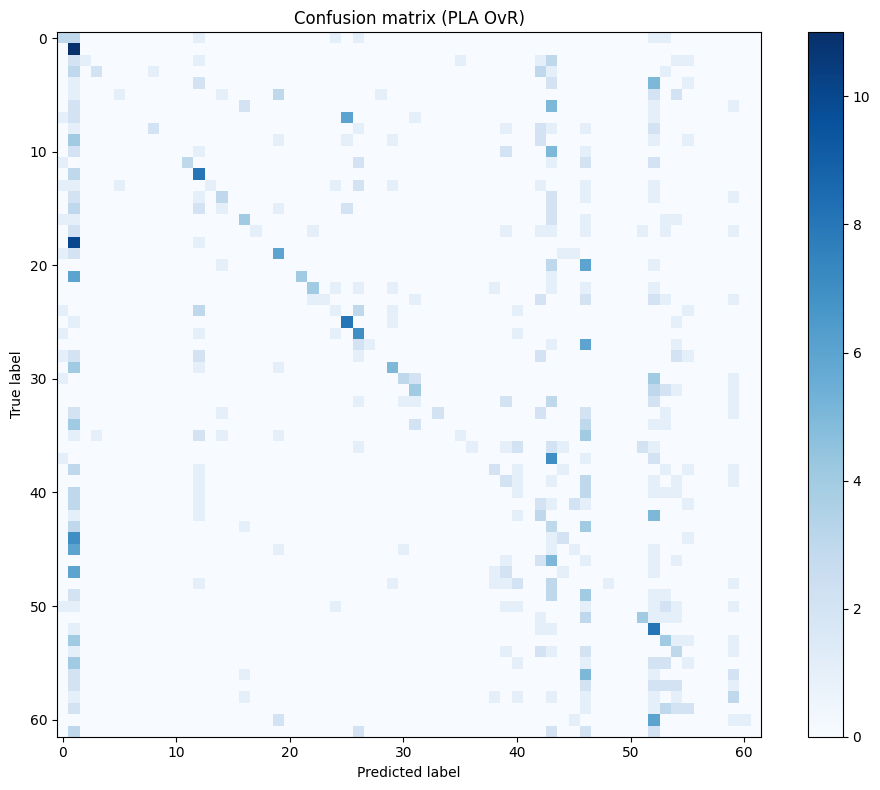
\includegraphics[width=0.75\linewidth]{MLP_images/cn_matrix.png}
  \caption{Confusion matrix (MLP). Replace with the actual image file.}
  \label{fig:confmat_mlp}
\end{figure}

\begin{figure}[H]
  \centering
  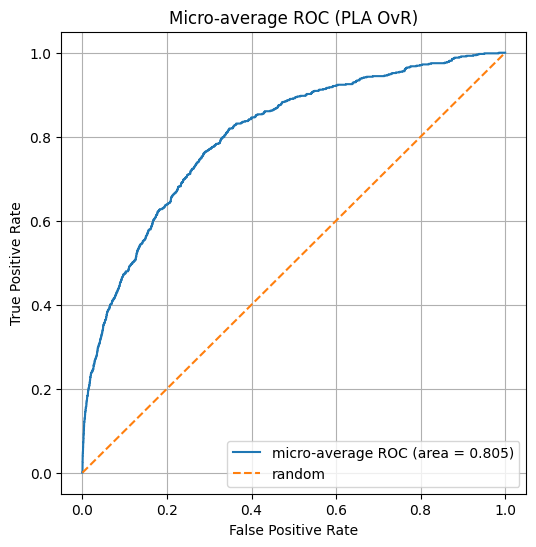
\includegraphics[width=0.75\linewidth]{MLP_images/roc.png}
  \caption{ROC curves (micro / macro). Replace with the actual image file.}
  \label{fig:roc_mlp}
\end{figure}

\begin{figure}[H]
  \centering
  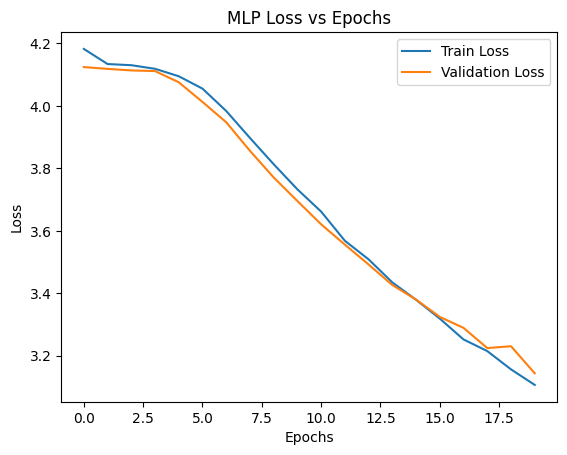
\includegraphics[width=0.75\linewidth]{MLP_images/mlp_loss.png}
  \caption{MLP Loss vs Epochs (training/validation).}
  \label{fig:mlp_loss}
\end{figure}

\begin{figure}[H]
  \centering
  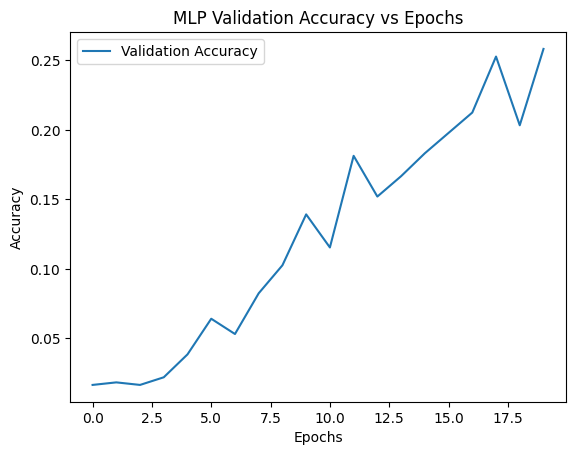
\includegraphics[width=0.75\linewidth]{MLP_images/mlp_acc.png}
  \caption{MLP Validation Accuracy vs Epochs.}
  \label{fig:mlp_val_acc}
\end{figure}

\section{Discussion}
\begin{itemize}
  \item The best MLP configuration achieved validation accuracy of \textbf{0.2582} via grid search.
  \item Test accuracy is \textbf{0.2317} with macro F1 approximately \textbf{0.1923}. Performance is limited, likely due to:
    \begin{itemize}
      \item Large number of classes (62) with relatively few examples per class (support=11 each in test).
      \item Balanced but small per-class supports — the model may overfit or under-generalize.
      \item MLP capacity and training schedule might need tuning (longer training, different architectures, or CNNs).
    \end{itemize}
  \item Several classes obtain very high recall but low precision or vice versa — suggests skewed predictions and class confusion for many classes.
\end{itemize}

\section{Conclusion}
The MLP baseline provides a working classifier and a grid-search-based tuning procedure. Accuracy and macro F1 are modest on this dataset; next steps should include stronger feature extractors (CNNs), augmentation, or per-class balancing strategies.



\end{document}
